\clearpage
\twocolumn[{%
\rqparent
\subsection{Item selection from the proxies alone}
\label{app:rq14_proxy_item_selection}

\noindent\begin{minipage}[t]{0.485\textwidth}
\vspace{0pt}
\paragraph{Research Question.} \emph{Can we shorten a benchmark using only the proxy runs, so that the short version still ranks the design variants as the 1.7B reference does on the full task?}

\paragraph{Setup.} We shorten each benchmark using only the proxy runs and measure the held-out DA-size of the kept items against the 1.7B ranking on the full task. We use the final checkpoints of the seed-1904 runs of every cell, ladder and data build that the per-item store holds (all but the twelve Muon runs at 90M--600M and the 1.7B K8 SwiGLU run). A pair may differ on any number of design axes, and a task must be above chance at the proxy and at 1.7B. We split the design families into two halves. On one half, we rank the items by their discrimination at 600M and 1B and keep the top quarter, half or three quarters of the candidates, the items whose outcome varies across those runs (about 36 \% of a task's items). An item's discrimination is the correlation of its correctness with the run's task score, both centred within each size. On the other half's pairs, we score the DA-size of the proxies 90M--1B on the kept items against the 1.7B ranking on the full task. Then the halves swap and we average the two readings. The baseline is random subsets of the same size, drawn from the same items. The selection never reads the 1.7B runs, so its DA is a held-out estimate that is available before the reference is trained. Only the task set, through the above-chance gate at 1.7B that every DA uses, depends on the reference.
\end{minipage}\hfill
\begin{minipage}[t]{0.485\textwidth}
\vspace{0pt}
\begin{rqfinding}
\textbf{1. The top half of the candidates is barely better than random items.} At q = 50 \% (about 18 \% of a task's items), the proxy-chosen items reach 0.490 at 90M to 0.554 at 1B, and random items 0.484 to 0.538. (Figure~\ref{fig:app_rq14_proxy_item_selection}.)
\\
\\
\textbf{2. Neither subset reaches the full task.} The full task reaches 0.528 at 90M to 0.571 at 1B, which is 0.013--0.038 above the proxy-chosen half.
\\
\\
\textbf{3. The gain over random is positive almost everywhere, but small.} It is positive in 14 of the 15 (q, size) cells and never above +0.017.
\end{rqfinding}
\end{minipage}

\vspace{\baselineskip}
\noindent\begin{minipage}{\textwidth}
\centering
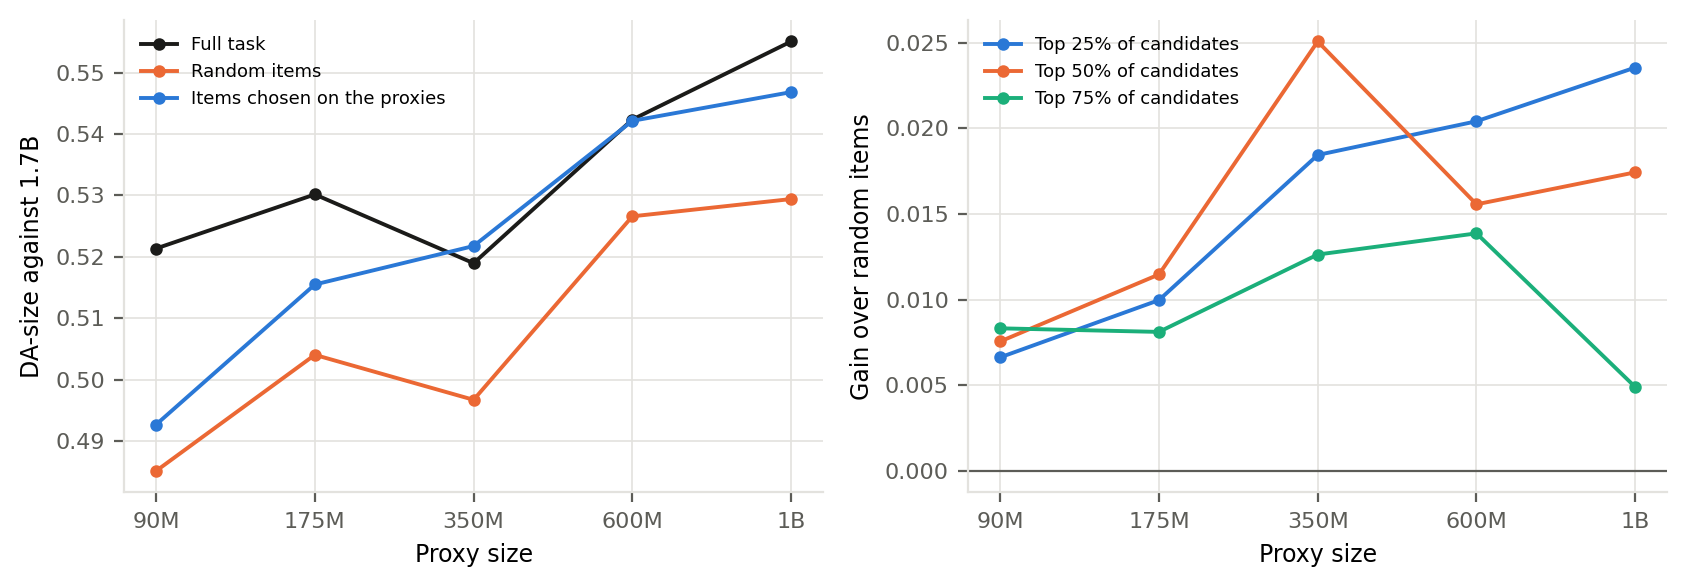
\includegraphics[width=\textwidth,height=0.36\textheight,keepaspectratio]{figures/app_rq14_proxy_item_selection.png}
% source: src/signal-and-noise/analysis/rq14_proxy_item_selection/pretraining/predictivity/proxy_item_selection_da_size_multi_axes_paper.png
\captionof{figure}{\textbf{The top half of the candidates is barely better than random items.} Left: DA-size of the proxies against the 1.7B ranking on the full task, on multi-axis design pairs, for the full task (black), for random items of the same count (orange) and for the top half of the items chosen on the proxies (blue). Right: the gain of the chosen items over the random ones, one line per share of the items kept.}
\label{fig:app_rq14_proxy_item_selection}
\end{minipage}
}]
